%%%%%%
%
% $Author: Wings $
% $Project:  $
% $Filename: BluetoothNinaB306.tex $
% $Short description: Entwicklerdokumentation Kapitel über das auf dem Arduino verbaute BLE Modul NinaB306 inkl. Beispiel Code $
%
%%%%%%

\chapter{Bluetooth Low Energy Modul Nina B306}

Das \textbf{NINA B306} Modul, von u-blox, ist ein Bluetooth Low Energy (BLE) Modul, das im Arduino Nano 33 BLE Sense integriert ist. Es basiert auf der Bluetooth-Generation 5.0 und ermöglicht drahtlose Kommunikation mit Smartphones und anderen BLE-fähigen Geräten. \cite{ublox:2017}

Bluetooth Low Energy (BLE) ist eine stromsparende Funktechnologie, die speziell für das Internet der Dinge (IoT) entwickelt wurde. Sie ermöglicht energieeffiziente Kommunikation über kurze Distanzen (typisch 1–10 m) und wird in Geräten eingesetzt, die mit Batteriebetrieb über lange Zeiträume arbeiten sollen. \cite{Kumar.2023}

\section{Wichtige Elemente eines BLE Moduls}
Ein typisches BLE Modul kombiniert folgende Komponenten:

\begin{itemize}
	\item \textbf{Mikrocontroller (MCU)} verarbeitet Nutzdaten und steuert den BLE-Stack.
	\item \textbf{HF Teil (Radio)} sendet und empfängt Signale im 2.4 GHz ISM-Band.
	\item \textbf{Firmware} enthält die BLE-Protokolle wie GAP, GATT, Link Layer.
	\item \textbf{Schnittstellen} z.B. UART oder SPI zur Anbindung an Mikrocontroller.
\end{itemize}
\cite{Morais.2023}

Module wie das \textbf{NINA-B306} enthalten bereits alle Komponenten in einem Gehäuse. \cite{ublox:2017}

	\subsection{Vorteile von BLE}
	BLE ist speziell für Anwendungen mit geringem Datenaufkommen und langer Batterielaufzeit konzipiert. Zu den zentralen Merkmalen gehören:
	
	\begin{itemize}
		\item \textbf{Geringer Energieverbrauch:} Geräte bleiben im Tiefschlaf und senden nur bei Bedarf.
		\item \textbf{Schneller Verbindungsaufbau:} Durch „Advertising“ werden Geräte sofort gefunden.
		\item \textbf{Sicher:} Unterstützt moderne Verschlüsselung (z.B. AES-128) und sicheres Pairing.
		\item \textbf{Flexibles Netzwerkmodell:} BLE unterstützt Punkt zu Punkt, Broadcasting und Mesh.
	\end{itemize}

	Diese Eigenschaften machen BLE ideal für IoT-Anwendungen wie Sensorik, Wearables, Fernsteuerungen und smarte Umgebungen.
	\cite{Kumar.2023}

	\subsection{BLE Stack}
	Der \textbf{BLE Stack} (Bluetooth Low Energy Stack) ist die zentrale Softwarestruktur, die die gesamte Kommunikation eines BLE Geräts steuert. Er besteht aus zwei Hauptkomponenten:

	\begin{itemize}
		\item Der \textbf{Host} verwaltet die höheren Protokolle wie GATT, GAP, ATT und L2CAP und ist für die Datenverarbeitung und Strukturierung zuständig.
		\item Der \textbf{Controller} ist für die physikalische Funkübertragung sowie das Link Layer verantwortlich.
	\end{itemize}

	Die Kommunikation zwischen Host und Controller erfolgt über das standardisierte \textbf{Host Controller Interface (HCI)}. Dieses Schnittstellenprotokoll regelt den Datenaustausch und die Steuerbefehle zwischen den beiden Komponenten.
	
	Für Entwickler bietet der BLE-Stack eine große Erleichterung: Durch die Bereitstellung standardisierter Schnittstellen lassen sich komplexe Bluetooth-Funktionen über einfache Programmbefehle nutzen  ohne tief in die Protokolldetails einsteigen zu müssen. \cite{Kumar.2023}
	
	
\begin{center}

\begin{tikzpicture}
	% Application Block
	\draw[black, fill=green!30, rounded corners] (0.5,-0.25) rectangle (13.5,1.75);
	\node[black, align=center] at ($(0.5,-0.25)!.5!(13.5,1.75)$) {
		Application \\
		Profiles and Services
	};
	
	% Host Block
	\draw[black!90, fill=cyan!30!blue!50, rounded corners] (0.5,-1) rectangle (13.5,-9.5);
	\node[black, align=center, font=\Large\bfseries] at (7,-2) {Host};
	
	% GATT Block
	\draw[black!90, fill=LightBlue!50, rounded corners] (1,-3) rectangle (5.5,-4.5);
	\node[black, align=center] at ($(1,-3)!.5!(5.5,-4.5)$) {
		Generic Attribute \\
		Profile (GATT)
	};
	
	% GAP Block
	\draw[black!90, fill=LightBlue!50, rounded corners] (6,-3) rectangle (12.5,-4.5);
	% Erweiterung GAP senkrecht
	\draw[black!90, fill=LightBlue!50, rounded corners] (11,-3) rectangle (12.5,-8.5);
	% Verbindungsstreifen GAP vertikal
	\draw[LightBlue!50, fill=LightBlue!50] (10.9,-3.01) rectangle (11.02,-4.49);
	\node[black, align=center] at ($(6,-3)!.5!(12.5,-4.5)$) {
		Generic Access Profile \\
		(GAP)
	};
	
	% ATT Block
	\draw[black!90, fill=LightBlue!50, rounded corners] (1,-5) rectangle (5.5,-6.5);
	\node[black, align=center] at ($(1,-5)!.5!(5.5,-6.5)$) {
		Attribute Protocol \\
		(ATT)
	};
	
	% SM Block
	\draw[black!90, fill=LightBlue!50, rounded corners] (6,-5) rectangle (10.5,-6.5);
	\node[black, align=center] at ($(6,-5)!.5!(10.5,-6.5)$) {
		Security Manager \\
		(SM)
	};
	
	% L2CAP Block
	\draw[black!90, fill=LightBlue!50, rounded corners] (1,-7) rectangle (10.5,-8.5);
	\node[black, align=center] at ($(1,-7)!.5!(10.5,-8.5)$) {
		Logical Link Control and Adaptation \\
		Protocol (L2CAP)
	};
	
	% Controller Block
	\draw[black!90, fill=gray!50, rounded corners] (0.5,-10.25) rectangle (13.5,-16);
	\node[black, align=center, font=\Large\bfseries] at (7,-15.25) {Controller};
	
	% Link Layer (LL) Block
	\draw[black!90, fill=gray!20, rounded corners] (1,-11) rectangle (12.5,-12.5);
	\node[black, align=center] at ($(1,-11)!.5!(12.5,-12.5)$) {
		Link Layer (LL)
	};
	
	% Physical Layer (PHY) Block
	\draw[black!90, fill=gray!20, rounded corners] (1,-13) rectangle (12.5,-14.5);
	\node[black, align=center] at ($(1,-13)!.5!(12.5,-14.5)$) {
		Physical Layer (PHY)
	};
	
	% HCI Block (blaugrau, zentriert)
	\draw[black!90, fill=blue!20!gray!40, rounded corners] (1,-9) rectangle (12.5,-10.5);
	\node[black, align=center] at ($(1,-9)!.5!(12.5,-10.5)$) {
		Host Controller Interface (HCI)
	};
\end{tikzpicture}
	
	\captionof{figure}[BLE Stack]{Darstellung des BLE Stack \cite{Tosi.2017} \cite{Morais.2023}}  
	\label{fig:BLEStack} 
\end{center}


\subsubsection{Elemte des BLE Stack}
Für den Aufbau des BLE Stack siehe \autoref{nRFStart}. Eine genauere Erläuterung der einzelnen Komponenten ist in der folgenden Auflistung zu finden.
\begin{itemize}
	\item \textbf{Application Layer (APP)}  Diese oberste Ebene stellt die Benutzeranwendung dar. Hier werden BLE-Profile implementiert, die Interoperabilität zwischen verschiedenen Geräten und Anwendungen sicherstellen.
	
	\item \textbf{GAP (Generic Access Profile)}  Regelt die grundlegenden BLE-Funktionen wie Sichtbarkeit, Rollenverteilung (z.\,B. Central/Peripheral) und Sicherheitsstufen. Ist Teil des Hosts und stellt die Verbindung zur Anwendungsschicht her.
	
	\item \textbf{GATT (Generic Attribute Profile)}  Verwaltet, wie strukturierte Daten (Services und Characteristics) organisiert, dargestellt und ausgetauscht werden. GATT baut auf ATT auf.
	
	\item \textbf{ATT (Attribute Protocol)}  Protokoll zum Lesen, Schreiben und Übertragen von Datenattributen über eine bestehende Verbindung. Dient als Basis für die GATT-Schicht.
	
	\item \textbf{SMP (Security Manager Protocol)}  Verwaltet Authentifizierung, Pairing und Verschlüsselung mit BLE spezifischen Sicherheitsmechanismen.
	
	\item \textbf{L2CAP (Logical Link Control and Adaptation Protocol)} Diese Schicht ist zuständig für die Weiterleitung und Aufteilung der Daten. Sie verpackt Informationen aus höheren Schichten in BLE-Pakete zum Senden und entpackt sie beim Empfang. Außerdem verteilt sie die Daten an die richtigen Stellen innerhalb des Hosts..
	
	\item \textbf{HCI (Host Controller Interface)}  Schnittstelle zwischen Host und Controller. Übersetzt Befehle und Ereignisse in beide Richtungen.
	
	\item \textbf{LL (Link Layer)}  Teil des Controllers. Regelt Paketformatierung, Timing, Verbindungsaufbau, Kanalauswahl und Fehlerkorrektur. 
	
	\item \textbf{PHY (Physical Layer)}  Unterste Ebene des Stacks. Führt die tatsächliche Funkübertragung im 2{,}4\,GHz-Band durch und definiert Modulation, Kanäle und HF-Charakteristika.
\end{itemize}
\cite{Tosi.2017} \cite{Morais.2023}

\section{NINA B306}

\section{Spezifikation}
\begin{longtable}{|p{5cm}|p{8cm}|}
	\caption{Spezifikationen Bluetooth-Modul NINA-B306}
	\label{tab:specs_nina_b306} \\
	
	\hline
	\multicolumn{2}{|l|}{\textbf{Hauptmerkmale}} \\
	\hline
	Modell & u-blox NINA-B306 \\
	\hline
	Chipsatz & Nordic Semiconductor nRF52840 \\
	\hline
	Abmessungen & 10 × 15 mm \\
	\hline
	Betriebstemperatur & –40 °C bis +85 °C \\
	\hline
	
	\multicolumn{2}{|l|}{\textbf{Weitere Spezifikationen}} \\
	\hline
	Bluetooth-Version & 5.0 Low Energy (BLE) \\
	\hline
	Frequenzbereich & 2.4 GHz ISM-Band, IEEE 802.15.4, proprietäre Modi \\
	\hline
	Maximale Datenrate & 2 Mbps \\
	\hline
	Schnittstellen & UART, SPI, GPIO, ADC \\
	\hline
	Versorgungsspannung & 1.7 V – 3.6 V \\
	\hline
	Stromverbrauch & 4.8 mA beim Senden (0 dBm) \\
	\hline
\end{longtable}

\cite{ublox:2017}

\begin{center}
	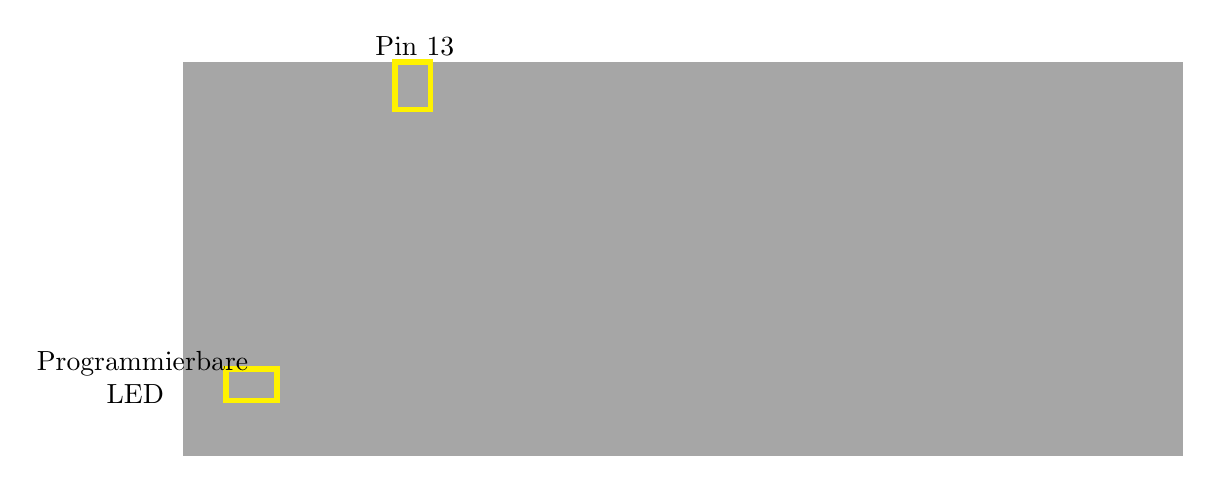
\begin{tikzpicture}
		
		\ArduinoNanoBLESenseRev;
		
		\fill[gray, opacity=0.7] (-0.2,0) rectangle (12.5,5.0);
		
		\coordinate (A) at (2.5,4.4);
		\coordinate (B) at (2.95,5); 
		
		
		\coordinate (C) at (1,0.7);
		\coordinate (D) at (0.35,1.1);   
		
		\def\cliparea{(C) rectangle (D); (A) rectangle (B); }  
		
		\begin{scope}
			\clip (C) rectangle (D);
			
			\ArduinoNanoBLESenseRev;
			
		\end{scope}
		
		\PINNO{2};
		
		\draw[yellow,line width=2pt] (A)  rectangle (B);
		\draw[yellow,line width=2pt] (C)  rectangle (D);
		
		\node (P25) at (2.75, 5.2) {Pin 13};
		\node (LED) at (-0.8, 1) [text width=2.5cm, align=center] {Programmierbare LED};
	\end{tikzpicture}    
	\captionof{figure}{Programmierbare LED des Arduinos Nano 33 BLE Sense}  
\end{center}


\section{Kalibrierung}
Das NINA-B306 Bluetooth Modul wird werksseitig von u-blox kalibriert und benötigt keine Kalibrierung.\cite{ublox:2017}

\subsection{Konfiguration}
Das NINA-B306 Modul von u-blox ist ein vorkonfiguriertes Bluetooth Low Energy (BLE) Modul auf Basis des nRF52840. Für eine effektive Integration in Arduino Projekte sind vor allem folgende Konfigurationen relevant:
Die wichtigsten Konfigurationsparameter für den praktischen Einsatz sind:
\begin{itemize}
	\item Name des BLE Geräts
	\item Sendeleistung (Reichweite vs. Stromverbrauch)
	\item Werbeintervall (Reaktionszeit vs. Energieeffizienz)
\end{itemize}

Diese Parameter lassen sich vollständig mit der \texttt{ArduinoBLE} Bibliothek auf dem Arduino Nano 33 BLE Sense konfigurieren. 
\cite{Arduino.2025c}

\subsubsection{Kommunikationsschnittstelle}
Das Modul kommuniziert  über eine UART-, SPI- oder USB Schnittstelle mit dem Host Mikrocontroller. Beim Einsatz auf dem Arduino Nano 33 BLE Sense erfolgt die Anbindung direkt über interne Kanäle,  es werden keine separate Schnittstellenkonfigurationen benötigt

\subsubsection{Betriebsmodus: BLE Peripheral}
Für typische Sensoranwendungen wird das Modul als \textbf{BLE Peripheral} betrieben. Dabei sendet das Modul regelmäßig Advertising Pakete aus und ermöglicht eine Verbindung mit zentralen Geräten (z.B. Smartphone oder PC).

\PYTHON{BLE.setLocalName("Sensor");}

\PYTHON{BLE.advertise();}

\subsubsection{Sendeleistung (TX Power)}
Die Ausgangsleistung des Funkmoduls kann zur Anpassung von Reichweite und Energieverbrauch justiert werden. Möglich sind Werte von –40 dBm bis +4 dBm.

\PYTHON{BLE.setTxPower(0);} (0 dBm, Standardwert)

\subsubsection{Advertising Intervall}
Die Frequenz, mit der das Modul Werbung (Advertising) sendet, beeinflusst sowohl die Reaktionszeit als auch den Energieverbrauch. Ein typischer Wert:

\PYTHON{BLE.advertiseInterval(1000);} (1000 ms)

\cite{ublox:2017}

\section{Bibliothek ArduinoBLE.h}
	\subsubsection{Beschreibung}
	Die \texttt{ArduinoBLE} Bibliothek ist eine offizielle Arduino Bibliothek, mit der sich Bluetooth Low Energy (BLE) einfach auf kompatiblen Boards wie dem Arduino Nano 33 BLE Sense nutzen lässt. Sie übernimmt die komplexe Kommunikation im Hintergrund und stellt leicht verständliche Befehle zur Verfügung, mit denen man BLE Funktionen schnell im eigenen Programm verwenden kann.
	\cite{Arduino.2025c}

	\begin{table}[H]
		\centering
		\begin{tabular}{|l|c|p{8cm}|}
			\hline
			\textbf{Bibliothek} & \textbf{Version} & \textbf{Beschreibung} \\
			\hline
			\textbf{ArduinoBLE.h} & \textbf{1.2.0} & Ermöglicht die Nutzung von Bluetooth Low Energy (BLE) auf unterstützten Arduino-Boards wie dem Nano 33 BLE Sense. Unterstützt sowohl Peripheral als auch Central-Funktionalität sowie das Erstellen und Verwalten von BLE Eigenschaften des BLE Moduls. \\
			\hline
		\end{tabular}
		\captionof{table}{Verwendete Bibliothek für das Bluetooth-Modul NINA-B306.}
	\end{table}

	\subsubsection{Installation}
	Die Bibliothek kann direkt über den Arduino Library Manager installiert werden:
	Näheres dazu in  \autoref{HowToLibrary}.
	
	\subsubsection{Relevante Funktionen}
	\begin{table}[H]
		\centering
		\begin{tabularx}{\textwidth}{|p{4.5cm}|X|}
			\hline
			\textbf{Funktion} & \textbf{Beschreibung} \\
			\hline
			\multicolumn{2}{|l|}{\textbf{Initialisierung und Konfiguration}} \\
			\hline
			\PYTHON{BLE.begin()} & Initialisiert den BLE-Stack und aktiviert das Bluetooth-Modul. Muss im \texttt{setup()} aufgerufen werden. \\
			\hline
			\PYTHON{BLE.setLocalName ("Name")} & Setzt den Gerätenamen, der beim Scannen sichtbar ist. \\
			\hline
			\PYTHON{BLE.advertise()} & Startet das BLE-Werbesignal, um Verbindungen zu ermöglichen. \\
			\hline
			\PYTHON{BLE.stopAdvertise()} & Beendet das Advertising. \\
			\hline
			\multicolumn{2}{|l|}{\textbf{Zentralgeräte-Funktionen (Central Role)}} \\
			\hline
			\PYTHON{BLE.scan()} & Startet den Scan nach verfügbaren BLE-Geräten. \\
			\hline
			\PYTHON{BLE.available()} & Prüft, ob ein Gerät im Scan gefunden wurde. \\
			\hline
			\PYTHON{BLEDevice peripheral = BLE.available()} & Greift auf ein gefundenes Gerät zu. \\
			\hline
			\multicolumn{2}{|l|}{\textbf{Verbindungs-Management}} \\
			\hline
			\PYTHON{BLE.connected()} & Prüft, ob aktuell eine Verbindung zu einem Gerät besteht. \\
			\hline
			\PYTHON{BLE.disconnect()} & Trennt eine bestehende Verbindung. \\
			\hline
			\PYTHON{BLE.central()} & Gibt das aktuell verbundene Zentralgerät als \texttt{BLE Device} zurück, sobald eine Verbindung aufgebaut wurde. Ermöglicht Zugriff auf Geräteinformationen wie Adresse oder Name. \\
			\hline
			\multicolumn{2}{|l|}{\textbf{Datenübertragung}} \\
			\hline
			\PYTHON{char.writeValue (value)} & Sendet einen Wert (z.B. Sensorwert) an das verbundene Gerät. \\
			\hline
			\PYTHON{char.readValue()} & Liest den aktuellen Wert der Charakteristik aus. \\
			\hline
		\end{tabularx}
		\captionof{table}{Verwendete Funktionen der \texttt{ArduinoBLE} Bibliothek im Projekt mit dem NINA B306 Modul.}
	\end{table}

	\textbf{Aufgaben und Funktionen der Bibliothek:}
	\begin{itemize}
		\item Initialisierung des BLE-Stacks und des Funkmoduls
		\item Verwaltung der BLE-Betriebsrollen:
		\begin{itemize}
			\item \textbf{Peripheral}: Gerät sendet Daten (z.\,B. Sensor)
			\item \textbf{Central}: Gerät empfängt/verbindet sich (z.\,B. Smartphone)
		\end{itemize}
		\item Erstellung und Verwaltung von BLE Services und Charakteristika
		\item Unterstützung für BLE-Werbung (advertising), Benachrichtigungen (notifications) und Datenübertragung (read/write)
	\end{itemize}


	\section{Codebeispiel}
	
	\subsection{Einfaches Beispiel mit Code BLE Advertising aktivieren }
	
	Das folgende Arduino Programm initialisiert das Bluetooth Low Energy (BLE) Modul und startet den \textbf{Advertising Modus}, wodurch das Gerät für BLE fähige Zentralgeräte sichtbar wird. 
	
	Mit der Smartphone App nRF Connect for Mobile  kann das Gerät unter dem angegebenen Namen \textbf{TestBLE} erkannt und angezeigt werden.
	
	\subsection{nRF Connect for Mobile}
	\label{sec:nrfconnect}
	Die App \textbf{nRF Connect for Mobile }ist kostenlos über die offiziellen App Stores von Apple und Google verfügbar:
	\begin{figure}[H]
		\centering
		
\includegraphics[width=6cm]{Bluetooth/NRFConnectLogo}
		\caption{Logo nRF connect for Mobile}
		\label{fig:nRFLogo}
	\end{figure}
	
	\begin{itemize}
		\item \textbf{Für Android:} \href{https://play.google.com/store/apps/details?id=no.nordicsemi.android.mcp}{nRF Connect im App Store}
		\item \textbf{Für iOS:} \href{https://apps.apple.com/gb/app/nrf-connect-for-mobile/id1054362403}{nRF Connect im App Store}
	\end{itemize}
	
	Nach dem Download ist die App sofort einsatzbereit. 
	\subsubsection{Benutzung}
	Starten Sie die App. Im oberen rechten Bereich Starten sie über die Schaltfläche \menu{scan } die Suche nach Bluetooth Ggeräten \autoref{fig:nRFStart}
	
	\begin{figure}[H]
		\centering
		\begin{tikzpicture}
			\node[anchor=south west, inner sep=0] (img) at (0,0) 	{
\includegraphics[width=6cm]{Bluetooth/NrfConnectStart}};
			\draw[red, line width=1pt] (4.8,3) rectangle (5.4,3.5);
			\node[red] at (5,3.8) {\tiny Scan starten};
		\end{tikzpicture}
		\caption{Oberfläche von nRF Connect for Mobile  Scan Schaltfläche}
		\label{fig:nRFStart}
	\end{figure}

	Im Anschluss Erscheint das Gerät unter dem Namen \textbf{TestBLE} in der Liste.
	
			\begin{figure}[H]
		\centering
		\begin{tikzpicture}
			\node[anchor=south west, inner sep=0] (img) at (0,0) 	{
\includegraphics[width=8cm]{Bluetooth/NRFConnectList}};
			\draw[red, line width=1pt] (0,5.5) rectangle (8,7.1);		
		\end{tikzpicture}
		\caption{Oberfläche von nRF Connect for Mobile  Geräteliste}
		\label{fig:nRFListe}
	\end{figure}
	
	\subsubsection{Funktionsweise des Codes:}
	\begin{itemize}
		\item Initialisiert die serielle Schnittstelle für Debug-Ausgaben.
		\item Startet das BLE-Modul über \PYTHON{BLE.begin()}.
		\item Setzt den lokalen Gerätenamen \textbf{TestBLE}.
		\item Aktiviert das BLE Advertising, sodass das Gerät sichtbar wird.
		\item Gibt eine Bestätigung in der IDE Konsole aus, zu sehen in Abbildung \autoref{MonitorBLEAdv}
	\end{itemize}
	
	\begin{figure}[H]
		\centering
		
\includegraphics[width=8cm]{Bluetooth/SerialMonitorBLEAdv}
		\caption{Serieller Monitor bestätigung start BLE Advertising}
		\label{fig:MonitorBLEAdv}
	\end{figure}
			
	{
		\captionof{code}{Testbeispiel zum Prüfen des Bluetooth (BLE) Advertising.}
		\label{Code:Test:File:TestBluetoothLowEnergy}
		\ArduinoExternal{}{../../Code/Nano33BLESense/Bluetooth/BLEAdver/BLEAdver.ino}
	}
	
	
	\subsection{Einfache Anwendung: Verbindungsaufbau}
	Dieses Beispielprogramm zeigt, wie eine Bluetooth Low Energy (BLE) Verbindung zwischen einem Arduino-Board und einem Zentralgerät (z.\,B. einem Smartphone mit \texttt{nRF Connect}) hergestellt und Informationen übertragen werden. Die App wird wie in \autoref{sec:nrfconnect} beschrieben verwendet. Anschließend wird über die Schaltfläche \menu{Connect}, siehe \autoref{nRFConnect}, die Verbindung mit dem Gerät aufgebaut. Zu sehen in \author{fig:nRFConnect}Danach wird die Adresse des mobilen Endgeräts angezeigt, von dem aus die Verbindung mit \texttt{nRF Connect} initiiert wurde. 


	
	\begin{figure}[H]
		\centering
		\begin{tikzpicture}
			\node[anchor=south west, inner sep=0] (img) at (0,0) 	{
\includegraphics[width=8cm]{Bluetooth/NRFConnectList}};			
			\draw[red, line width=1pt] (6,6) rectangle (8,6.9);				
		\end{tikzpicture}
		\caption{Oberfläche von nRF Connect for Mobile  Verbinden mit Gerät}
		\label{fig:nRFConnect}
	\end{figure}
	
	\subsubsection{Funktionsweise:}
	
	\begin{itemize}
		\item Initialisiert das BLE-Modul mit \PYTHON{BLE.begin()}.
		\item Setzt den Gerätenamen auf \textbf{TestBLE} und startet den Advertising Modus.
		\item Gibt in der seriellen Konsole aus, dass BLE Werbung gestartet wurde.
		\item Wartet auf eine Verbindung von einem Zentralgerät.
		\item Gibt beim Verbindungsaufbau die Adresse des verbundenen Geräts aus. Wie in \autoref{MonitorBLEAdresse} zu sehen.
		\item Überwacht kontinuierlich den Verbindungsstatus.
		\item Sobald die Verbindung getrennt wird, erfolgt eine entsprechende Meldung.
	\end{itemize}
	
	\begin{figure}[H]
		\centering
		
\includegraphics[width=10cm]{Bluetooth/SerialMonitorBLEAdress}
		\caption{Serieller Monitor Ausgabe der Adresse des verbundenen Gerätes}
		\label{fig:MonitorBLEAdresse}
	\end{figure}
	
	{
		\captionof{code}{Testbeispiel zum Prüfen des Bluetooth (BLE) Advertising.}
		\label{Code:Test:File:TestBluetoothLowEnergy}
		\ArduinoExternal{}{../../Code/Nano33BLESense/Bluetooth/BLEReadName/BLEReadName.ino}
	}
	
	
	\subsection{Beispielanwendung}
	Dieses Arduino-Programm ermöglicht die drahtlose Steuerung der internen LED eines \textit{Arduino Nano 33 BLE Sense} über die RemoteXY App mittels \textbf{Bluetooth Low Energy (BLE)}.
	
	\begin{enumerate}
		\item \textbf{Start \& Initialisierung}\\
		Beim Start initialisiert das Programm die RemoteXY Schnittstelle und konfiguriert den Pin der internen LED (\texttt{LED\_BUILTIN}) als Ausgang.
		
		\item \textbf{Bluetooth-Verbindung}\\
		Das Board wird unter dem Namen \texttt{RemoteXY} als BLE Gerät sichtbar. Die RemoteXY App auf dem Smartphone kann sich damit verbinden. Für eine Installationsanleitung Siehe \autoref{chap:RemoteXY}.
		
		\item \textbf{Benutzeroberfläche}\\
		In der App ist ein einziger Button verfügbar. \autoref{fig:RemoteXYButton} Die grafische Oberfläche wurde zuvor im RemoteXY-Editor erstellt und im Code als Byte-Array eingebettet (\texttt{RemoteXY\_CONF}). Siehe \autoref{chap:RemoteXY}.
		
		\item \textbf{LED-Steuerung}\\
		Wird der Button gedrückt, wird das Feld \texttt{button\_01} in der RemoteXY-Struktur auf \texttt{1} gesetzt. Das Hauptprogramm prüft diesen Zustand in der \texttt{loop()}-Funktion und:
		\begin{itemize}
			\item schaltet die LED \textbf{ein}, wenn der Button gedrückt ist, 
			\item schaltet sie \textbf{aus}, wenn der Button losgelassen wird.
		\end{itemize}
		Die LED ist in \autoref{fig:ArduinoLED} abgebildet. Sie ist mit dem Pin 13 verbunden.
	\end{enumerate}

	\subsubsection{Beispiel Code}
	{
		\captionof{code}{Testbeispiel zum Prüfen der Bluetooth (BLE) verbindung eines Mobilen Endgerätes mit dem Arduino.}
		\label{Code:Test:File:TestBluetoothLowEnergy}
		\ArduinoExternal{}{../../Code/Nano33BLESense/Bluetooth/BLEBlink/BLEBlink.ino}
	}

\begin{center}
  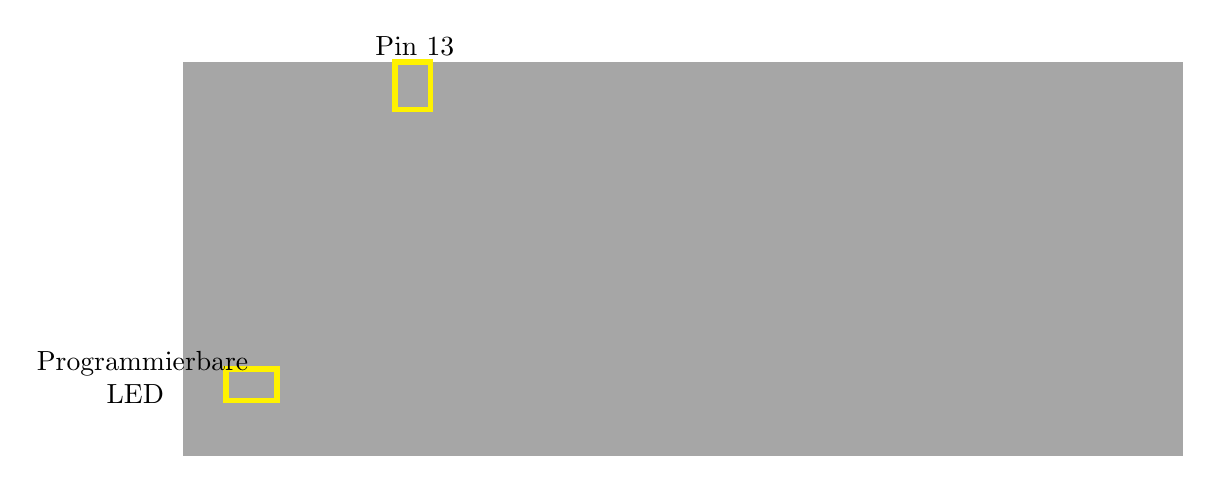
\begin{tikzpicture}
	
	\ArduinoNanoBLESenseRev;
	
	\fill[gray, opacity=0.7] (-0.2,0) rectangle (12.5,5.0);
	
	\coordinate (A) at (2.5,4.4);
	\coordinate (B) at (2.95,5); 
	
	
	\coordinate (C) at (1,0.7);
	\coordinate (D) at (0.35,1.1);   
	
	\def\cliparea{(C) rectangle (D); (A) rectangle (B); }  
	
	\begin{scope}
		\clip (C) rectangle (D);
		
		\ArduinoNanoBLESenseRev;
		
	\end{scope}
	
	\PINNO{2};
	
	\draw[yellow,line width=2pt] (A)  rectangle (B);
	\draw[yellow,line width=2pt] (C)  rectangle (D);
	
	\node (P25) at (2.75, 5.2) {Pin 13};
	\node (LED) at (-0.8, 1) [text width=2.5cm, align=center] {Programmierbare LED};
  \end{tikzpicture}    
  \captionof{figure}{Arduino Nano 33 BLE Sense Beispiel BLE} \label{fig:ArduinoLED}
\end{center}

	
\begin{center}
  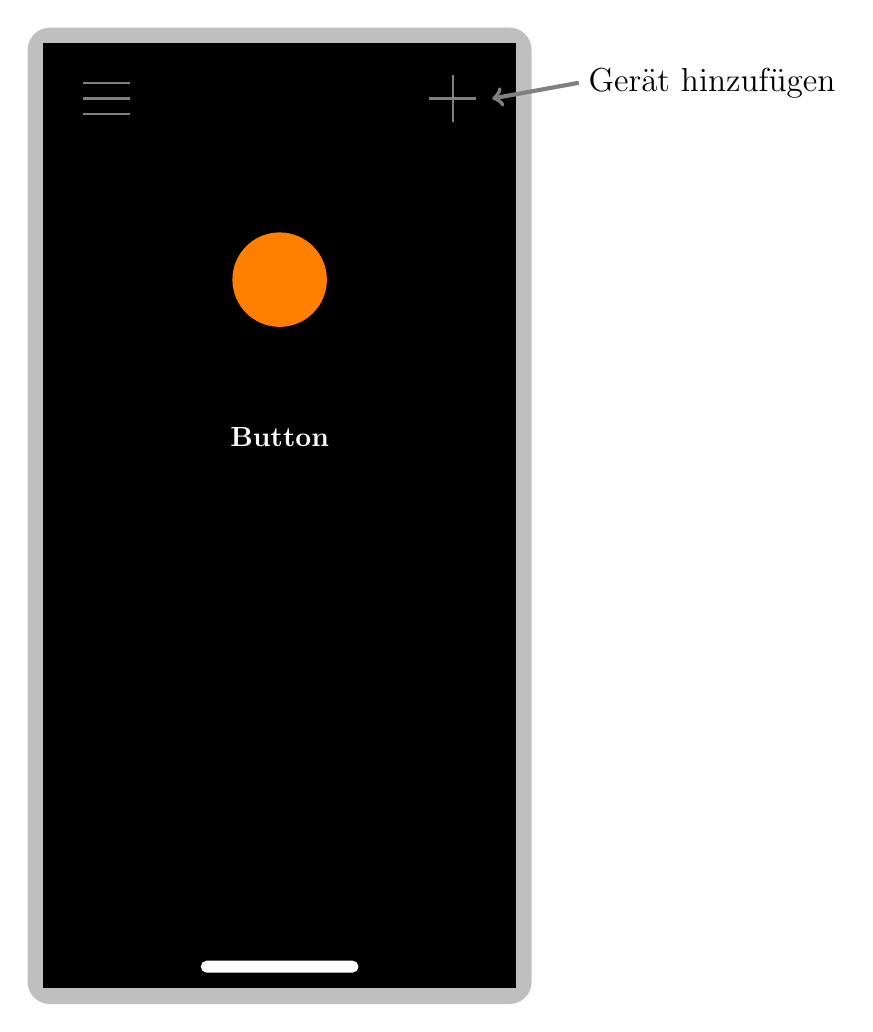
\begin{tikzpicture}
	
	% Gehäuse des "Smartphones" mit abgerundeten Ecken (dünner Rahmen)
	\fill[gray!50, rounded corners=8pt] (-0.2,-0.2) rectangle (6.2,12.2);
	
	% Hintergrund des Displays
	\fill[black] (0,0) rectangle (6,12);
	
	% Schmales Rechteck (Home-Bar) am unteren Rand
	\fill[white, rounded corners=2pt] (2,0.2) rectangle (4,0.35);
	
	% Menü-Icon (oben links): Drei kleine graue Linien 
	\draw[gray, line width=0.8pt] (0.5,11.5) -- (1.1,11.5);
	\draw[gray, line width=0.8pt] (0.5,11.3) -- (1.1,11.3);
	\draw[gray, line width=0.8pt] (0.5,11.1) -- (1.1,11.1);
	
	% Plus-Icon (oben rechts)
	\draw[gray, line width=0.8pt] (4.9,11.3) -- (5.5,11.3); % Horizontale Linie
	\draw[gray, line width=0.8pt] (5.2,11.6) -- (5.2,11.0); % Vertikale Linie
	
	% Umgedrehter Pfeil (von rechts nach links) leicht nach rechts verschoben
	\draw[<-, gray, line width=1.5pt]   (5.7,11.3) -- (6.8,11.5);
	\node[font=\large, anchor=west] at (6.8,11.5) {Gerät hinzufügen};
	
	\begin{scope}[shift={(3,9)}, rotate=90]	
		% Zentrum
		\fill[orange] (0,0) circle (0.6);
	\end{scope}
	
	% Beschriftung "Leistung"
	\node[white] at (3,7) {\textbf{Button}};
	
  \end{tikzpicture}	

  \captionof{figure}{Oberfläche von RemoteXY für das Testprogramm} \label{fig:RemoteXYButton}
	\end{center}


	\section{Weiterführende Literatur}
	
	\begin{itemize}
		\item \textbf{Bluetooth}  
		In dem Buch \textit{Connecting the Internet of Things: IoT Connectivity Standards and Solutions} von Anil Kumar finden sich in Kapitel 4 ausführliche Informationen zum Thema Bluetooth. Dabei werden unter anderem folgende Aspekte behandelt:
		
		\begin{itemize}
			\item Vergleich von Bluetooth Classic und Bluetooth Low Energy (BLE)
			\item Bluetooth Netzwerkmodelle
			\item Sicherheitsaspekte der Bluetooth-Kommunikation
			\item Anwendungsfälle und Einsatzgebiete in IoT Systemen
		\end{itemize}
		
		Diese Quelle bietet eine gute Grundlage, um das Verständnis für die Rolle von Bluetooth in drahtlosen Kommunikationssystemen zu vertiefen. \cite{Kumar.2023}
		
		\item \textbf{nRF52840 }  
		Die offizielle Dokumentation des Mikrocontrollers \textit{nRF52840} von Nordic Semiconductor ist eine zentrale Quelle für technische Details, Registerbeschreibungen und Architekturinformationen. Besonders hilfreich sind:
		
		\begin{itemize}
			\item Das Dokument bietet eine vollständige Beschreibung der \textbf{Kernkomponenten} des nRF52840, einschließlich CPU, Speicherarchitektur (RAM, Flash), EasyDMA, Debugschnittstellen und Konfigurationsregister (FICR, UICR).
			\item Es enthält detaillierte Informationen zur \textbf{Energieverwaltung}, z.B. zum Power Management Unit (PMU), Systemmodi (System ON/OFF), Stromverbrauch, Reset-Verhalten und der Taktsteuerung (HFCLK/LFCLK).
			\item Umfangreiche Kapitel zu den \textbf{Peripheriegeräten} beschreiben unter anderem die Funktionalität von GPIO, UART, ADC, SPI, I2C sowie sicherheitsrelevante Module wie CRYPTOCELL und CCM für Verschlüsselung.
			\item Zusätzlich werden die \textbf{elektrischen Eigenschaften und Grenzwerte} des Chips aufgeführt, etwa Spannungsbereiche, Stromverbrauch je Betriebsmodus sowie spezifische Anforderungen an externe Komponenten.
		\end{itemize}
		
		Die Dokumentation ermöglicht ein tiefgehendes Verständnis der Hardware, insbesondere wenn man den BLE Stack direkt nutzen möchte. Sie ist insbesondere für fortgeschrittene Projekte mit hoher Performance oder eigenem Protokolldesign relevant. \cite{NordicSemiconductor.2024}
		
		
		
		\item \textbf{Bluetooth 5.0 Spezifikation}  
		Die offizielle Bluetooth 5.0 Spezifikation der \textit{Bluetooth Special Interest Group (SIG)} bietet eine umfassende technische Beschreibung aller Funktionen, Protokolle und Anforderungen der BLE  Kommunikation. Sie bildet die Grundlage für moderne Anwendungen wie IoT-Geräte, Wearables, Smart Home und industrielle Sensorik.
		
		Die Spezifikation ist in mehrere Bände gegliedert, die verschiedene Aspekte des Systems detailliert behandeln:
		
		\begin{itemize}
			\item \textbf{Vol 0 – Compliance Requirements:} Definition grundlegender Produkttypen (z.\,B. Endprodukt, Subsystem), Konformitätsanforderungen und Kernkonfigurationen für z.\,B. BLE.
			\item \textbf{Vol 1 – Architekturübersicht:} Beschreibung der als Übersicht die Systemarchitektur, Datenflüsse, physikalischen Kanäle und Sicherheit. Enthält auch Details zu den Sicherheitsmechanismen für Datenverschlüsselung und Pairing.
			\item \textbf{Vol 2–4 – Core System:} Technische Spezifikationen der Basisbandfunktionen, des Link Managers, der Radio-Eigenschaften sowie der Host Controller Interfaces (HCI).
			\item \textbf{Vol 6 – Low Energy Specification:} Enthält die spezifischen Protokolle und Datenstrukturen für BLE.
			\item \textbf{Vol 7 – Wireless Coexistence:} Beschreibung von Mechanismen zur Koexistenz mit anderen Funksystemen wie WLAN.
		\end{itemize}
		
		Diese Spezifikation ist essenziell für Entwickler, die BLE Funktionalitäten korrekt und interoperabel implementieren möchten. Sie stellt sicher, dass BLE Geräte miteinander kompatibel sind und den festgelegten Standards entsprechen. \cite{BluetoothSpecialInterestGroup.2024}

		
	\end{itemize}



%%%%%%%%%%%%%%%%%%%%%%%%%%%%%%%%%%%%%%

\chapter{Bluetooth Low Energy Modul Nina B306}
\label{Nina}

\section{Einleitung}
Bluetooth Low Energy (BLE) hat sich als Standardtechnologie für drahtlose Kommunikation bei energieeffizienten Anwendungen etabliert. Typische Anwendungsfelder sind Wearables, Sensornetzwerke, IoT-Geräte und medizinische Systeme. In diesem Projekt kommt das BLE-Modul NINA-B306, integriert auf dem Arduino Nano 33 BLE Sense, zum Einsatz. Es ermöglicht die energieeffiziente Kommunikation mit mobilen Geräten oder anderen BLE-fähigen Systemen. \cite{Tosi:2017} \cite{UBLOX:2023}

\section{Grundlegende Informationen zu Bluetooth Low Energy}
Bluetooth Low Energy (BLE) ist eine energiesparende Funktechnologie, die mit Bluetooth 4.0 eingeführt wurde. Im Gegensatz zum klassischen Bluetooth fokussiert sich BLE auf Anwendungen, die eine geringe Datenrate benötigen, jedoch eine lange Batterielaufzeit erfordern. BLE arbeitet im 2,4-GHz-ISM-Band. BLE ist ideal für kleine Automatisierungsprojekte, die periodisch kleine Datenmengen senden.\cite{Tosi:2017} \cite{UBLOX:2023}
\subsection{ISM-Band}
Das ISM-Band (Industrial, Scientific and Medical Band) ist ein lizenzfreier Frequenzbereich, der weltweit für industrielle, wissenschaftliche und medizinische Anwendungen zur Verfügung steht. Für Bluetooth Low Energy wird das 2,4-GHz-ISM-Band verwendet, welches von 2400 - 2483,5 MHz reicht. Es stehen 40 Kanäle zur Verfügung, wobei 3 als Werbekanäle und 37 als Datenkanäle verwendet werden. BLE nutzt ein sogenanntes Frequency Hopping Spread Spectrum (FHSS), also ein Frequenzsprungverfahren, um Störungen zu minimieren und die Übertragung robuster zu machen.

\subsection{Datenraten}
Bluetooth Low Energy unterstützt verschiedene Datenraten, je nach Anwendungsbedarf:
\begin{itemize}
	\item 125 kBps: sehr energiesparend, geeignet für einfache Sensordaten
	\item 500 kBps: Guter Kompromiss zwischen Reichweite und Geschwindigkeit
	\item 1 MBps: Standard, geeignet für typische BLE-Anwendungen
	\item 2 MBps: Höchste Rate, schnelle Datenübertragung bei geringer Reichweite 
\end{itemize}
Die Datenrate beeinflusst den Stromverbrauch und die Reichweite. Eine hohe Datenrate verbraucht viel Energie und hat wenig Reichweite. \cite{Tosi:2017}

\subsection{Sendeleistung}
Die Sendeleistung (Output Power) gibt an, mit welcher Stärke ein Funksignal abgestrahlt wird. Sie wird in dBm (Dezibel bezogen auf 1 Milliwatt) angegeben. In Europa ist die maximal erlaubte Sendeleistung im 2,4 GHz ISM-Band ETSI-Normen geregelt und darf +20 dBm nicht überschreiten. \cite{ETSI:2004}

\section{BLE-Modul: NINA-B306-00B}
Das NINA-B306-00B ist ein Mitglied der u-blox NINA-B3-Serie, welches Bluetooth 5.0 Low Energy unterstützt. Es handelt sich um ein sogenanntes Open-CPU-Modul, d.h. es enthält einen eigenen Mikrocontroller (nRF52840 von Nordic Semiconductor), auf dem benutzerdefinierte Applikationen direkt ausgeführt werden können. Der Arduino Nano 33 BLE Sense nutzt dieses Modul zur BLE-Kommunikation. \cite{Tosi:2017} \cite{UBLOX:2023}

\section{Spezifikation}
\begin{itemize}
	\item Speicher: 1 MB Flash, 256 kB RAM
	\item Bluetooth-Version: Bluetooth 5.0 Low Energy
	\item Sendeleistung: +8 dBm
	\item Empfangsempfindlichkeit: -94 dBm (1 MB/s), 100 dBm (125 kB/s)
	\item Unterstützte Modi: BLE, IEEE 802.15.4, proprietäre 2,4-GHz-Protokolle
	\item Schnittstellen: UART, SPI, I2C, QSPI, I2S, USB 2.0, ADC (8-Kanal), PWM, GPIOs, NFC (passiv, nur als Tag)
	\item Bauform: 10 x 15 mm 
	\item Energieverwaltung: Sleep-, Standby- und aktiver Modus
	\item Zertifizierungen: CE, FCC, Bluetooth SIG
	\item Besonderheiten: Unterstützt Mesh-Netzwerke und sichere Boot-Funktion
\end{itemize}
 \cite{UBLOX:2023}
 
\section{Bibliothek}
Um die Kommunikation über Bluetooth Low Energy (BLE) mit dem Arduino Nano 33 BLE Sense zu realisieren, wird die Bibliothek \python{ArduinoBLE.h} (Version 1.4.0) benötigt. Diese Bibliothek stellt sämtliche Funktionen zur Verfügung, um BLE-Geräte zu konfigurieren und zu verbinden. Sie wurde speziell für Boards mit dem integrierten u-blox NINA-B3 Modul entwickelt.

Die Bibliothek ist bei der Installation der aktuellsten Version der Arduino-IDE (Version 2.3.6) in der Regel bereits enthalten. Sollte sie dennoch fehlen, kann sie wie folgt installiert werden:

\begin{itemize}
	\item Öffnen Sie die Arduino-IDE
	\item Gehen Sie zu \menu{Sketch > Bibliothek einbinden > Bibliotheken verwalten\ldots}
	\item Suchen Sie nach \menu{ArduinoBLE}
	\item Klicken Sie auf \menu{Installieren}
\end{itemize}

\section{Tests}
Man kann das BLE Modul testen, indem man den Arduino Nano 33 BLE Sense (Lite) einschaltet und mit der nRF-Connect-App BLE Geräte in der Nähe sucht. Detaillierte Informationen zu nRF-Connect sind im Kapitel \ref{chap:einstiegNRF} zu finden. Mit folgendem Code initialisiert man den Arduino für nRF-Connect und er wird sichtbar für die nRF-Connect-App: \ref{code:testBLE}

{
	\captionof{code}{Einfacher Code zum Testen von BLE}
	\label{code:testBLE}
    \ArduinoExternal{}{../../Code/Arduino/Bluetooth/BLETest/BLETest.ino}
}

Um sich auf der App mit dem Arduino zu verbinden sind folgende Schritte zu machen:
\menu{Gerät scannen/nach unten wischen > \glqq Nano33 BLE Test\grqq auswählen > Verbinden}
Danach sollte folgende Mitteilung auf dem Bildschirm erscheinen: \glqq BLE funktioniert!\grqq.

\section{Einfache Anwendung}
Als eine einfache Anwendung könnte man einen Lichtsensor mit Analogausgang mit dem Arduino verbinden. Dieser misst die einfallende Wellenlänge des Lichts und gibt diese grafisch auf der nRF-Connect-App aus. \ref{code:BLETest}

{
	\captionof{code}{Einfache Anwendung für BLE}
	\lstset{breaklines=true, breakatwhitespace=true}
	\label{code:BLETest}
	\ArduinoExternal{}{../../Code/Arduino/Bluetooth/BLEApp/BLEApp.ino}
}

Folgende Hinweise zum Code und der Anwendung:

\begin{itemize}
	\item \python{wavelenghtChar} sendet den Wert in Nanometern (zum Beispiel 500 nm = Grün)
	\item In der App kann der Live-Plot angezeigt werden, dazu das Graph-Symbol antippen
\end{itemize}

\section{Further Readings}

Heydon, Bluetooth Low Energy: The Developers Handbook, Prentice Hall, 2012 \cite{Heydon:2012}

\begin{itemize}
	\item Ein technisches Fachbuch direkt vom BLE-Mitentwickler. Es behandelt die Spezifikation, Architektur, Protokollstapel und Implementierungsdetails von BLE – mit Fokus auf tieferes Verständnis der Technologie.
\end{itemize} 

